\begin{figure}
\centering	
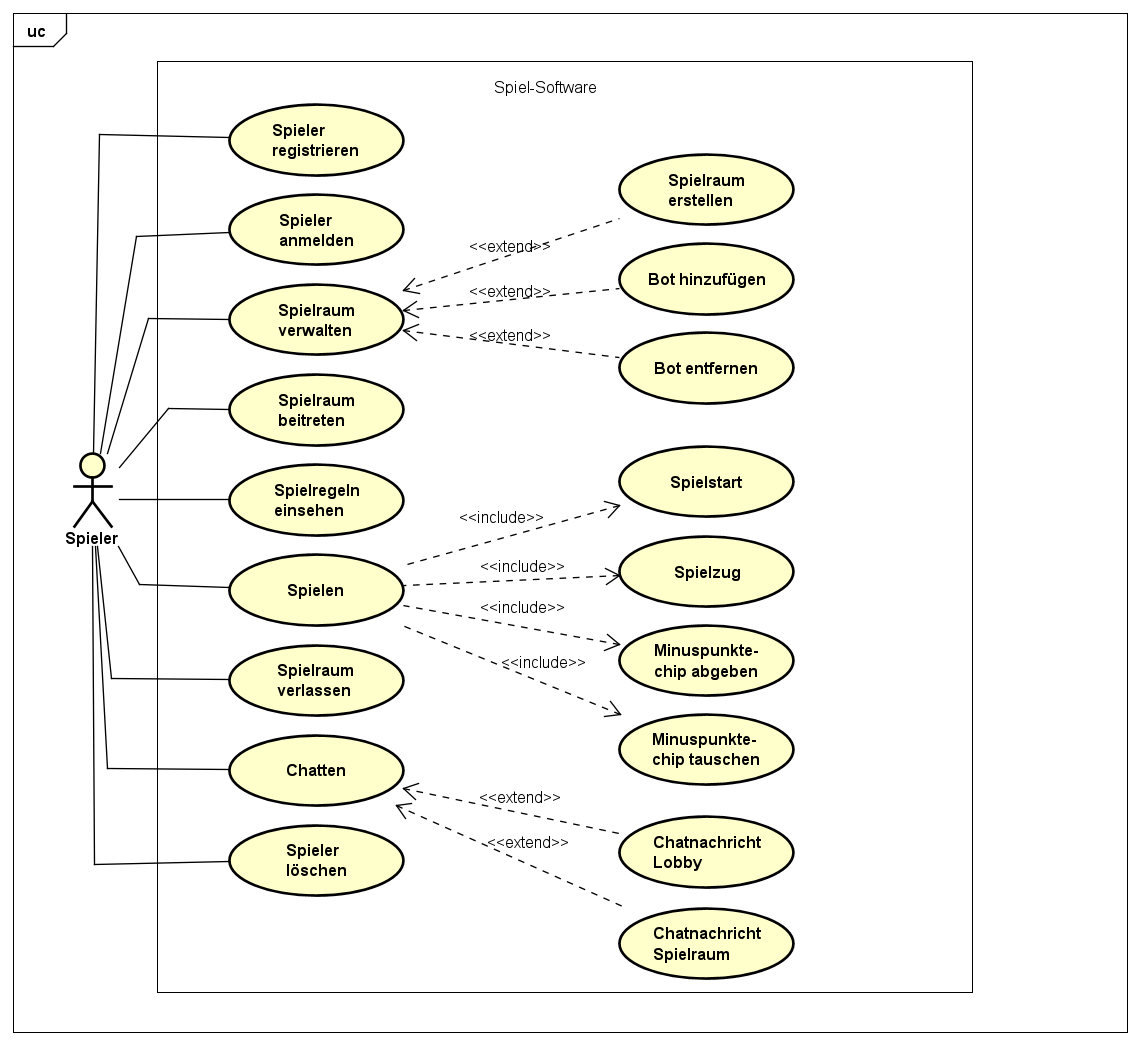
\includegraphics[width=0.9\textwidth]{img/ucd.png}
\label{fig:sys}
\caption{Systemgrenzendiagramm (Use Case Diagramm)}
\end{figure}

\section{Systemgrenze (Use Case Diagramm)}

Die Systemgrenze wird in der Abbildung~\ref{fig:sys} dargestellt\footnote{Weitere Erklärungen und Spezifizierungen, die sich auf Abgrenzungen der Verantwortlichkeiten vom System und weiteren Akteuren/Systemen beziehen, können hier spezifiziert werden.}. 


\section{Beschreibungen der Anwendungsfälle}

\newcounter{uc}\setcounter{uc}{10}

\begin{description}[leftmargin=5em, style=sameline]

	\begin{lhp}{uc}{UC}{uc:srerstellen}
		\item [Name:]Spielraum erstellen
		\item [Ziel:]Spieler erstellt einen Spielraum.
		\item [Akteure:]Spieler. 
		\item [Vorbedingungen:]Spieler befindet sich in der Lobby.
		\item [Eingabedaten:]Keine.
		\item [Beschreibung:]Ein Spieler erstellt einen neuen Spielraum.
		\item [Ausnahmen:]Keine.
		\item [Ergebnisse und Outputdaten:] Agierender Spieler befindet sich in einem neuen Spielraum, neuer Spielraum wird in der Lobby angezeigt.
		\item [Systemfunktionen:] \ref{funk:spielraum} 
	\end{lhp}
	
	\begin{lhp}{uc}{UC}{uc:srbeitreten}
		\item [Name:]Spielraum beitreten.
		\item [Ziel:]Spieler tritt Spielraum bei.
		\item [Akteure:]Spieler.
		\item [Vorbedingungen:]Spieler befindet sich in Lobby.
		\item [Eingabedaten:] Aktive Spielräume \ref{daten:spielräume}.
		\item [Beschreibung:]Spieler wählt einen aktiven Spielraum und tritt diesem bei.
		\item [Ausnahmen:]\hfill \begin{itemize} 
		\item[] 
		\textit{Spielraum bereits voll:} Eine entsprechende Fehlermeldung wird angezeigt, Spieler verbleibt in der Lobby.
		\item[]
		\textit{Spiel wurde bereits gestartet:} Eine entsprechende Fehlermeldung wird angezeigt, Spieler verbleibt in der Lobby.
		\end{itemize}
		\item [Ergebnisse und Outputdaten:] Spieler befindet sich im ausgewählten Spielraum.
		\item [Systemfunktionen:] \ref{funk:spielraum} 
	\end{lhp}
	
	\begin{lhp}{uc}{UC}{uc:spielregeln}
		\item [Name:]Spielregeln einsehen
		\item [Ziel:]Dem agierenden Spieler wird das gesamte Regelwerk angezeigt.
		\item [Akteure:]Spieler.
		\item [Vorbedingungen:]Der agierende Spieler befindet sich in der Lobby.
		\item [Eingabedaten:]Keine.
		\item [Beschreibung:]Jeder Spieler hat die Möglichkeit das LAMA-Regelwerk einzusehen.
		\item [Ausnahmen:]Keine.
		\item [Ergebnisse und Outputdaten:]Dem agierenden Spieler wird das LAMA-Regelwerk angezeigt. \ref{daten:spielregeln}
		\item [Systemfunktionen:]\ref{funk:regelwerk}
	\end{lhp}
	
	\begin{lhp}{uc}{UC}{uc:srverlassen}
		\item [Name:]Spielraum verlassen
		\item [Ziel:]Ein Spieler gelangt aus dem Spielraum zurück in die Lobby.
		\item [Akteure:]Spieler.
		\item [Vorbedingungen:]Spieler befindet sich in einem aktiven Spielraum.
		\item [Eingabedaten:]\ref{daten:spielräume}  
		\item [Beschreibung:]Spieler verlässt einen aktiven Spielraum und gelangt zurück in die Lobby.
		\item [Ausnahmen:]\hfill
		\begin{itemize}
		    \item[] \textit{Spiel wurde gestartet und noch nicht beendet: } agierender Spieler wird durch einen Bot ersetzt.
		    \item[] \textit{Agierender Spieler ist der letzte im Spielraum: }Spieler verlässt den Spielraum, dieser wird anschließend gelöscht.
		\end{itemize}
		\item [Ergebnisse und Outputdaten:] Spieler befindet sich in der Lobby, Spielraum wird ggf. gelöscht (siehe Ausnahmen).
		\item [Systemfunktionen:]  \ref{funk:spielverw}, \ref{funk:spielraum}, \ref{funk:bots}
	\end{lhp}
	
	\begin{lhp}{uc}{UC}{uc:spielzug}
		\item [Name:]Spielzug
		\item [Ziel:]Spieler führt einen Spielzug aus 
		\item [Akteure:]Spieler.
		\item [Vorbedingungen:]Der agierende Spieler befindet sich in einem aktiven Spiel und ist an der Reihe.
		\item [Eingabedaten:] \ref{daten:handkarten}, \ref{daten:stapelkarten}, \ref{daten:ablagestapel} 
		\item [Beschreibung:] Spieler führt einen der drei Spielzüge \dq Karte ablegen\dq, \dq Karte ablegen\dq\ und \dq Aussteigen\dq aus (vrgl. Regelwerk).
		\item [Ausnahmen:] \hfill
		\begin{itemize}
		    \item [] \textit{Spielzug ist ungültig:} Eine entsprechende Fehlermeldung wird angezeigt und der Spieler darf erneut einen Spielzug wählen.
		    
		    \item [] \textit{Spieler reagiert innerhalb von einer Minute nicht :} Ein beliebiger gültiger Spielzug wird ausgeführt.
		\end{itemize}
		\item [Ergebnisse und Outputdaten:] Spielzug wird ausgeführt und der nächste Spieler oder Bot ist an der Reihe. \ref{daten:handkarten}, \ref{daten:stapelkarten}, \ref{daten:ablagestapel}.
		\item [Systemfunktionen:]\ref{funk:spielverw}.
	\end{lhp}
	
	\begin{lhp}{uc}{UC}{uc:botspielzug}
		\item [Name:]Spielzug Bot
		\item [Ziel:]Bot schließt Spielzug ab.
		\item [Akteure:]System 
		\item [Vorbedingungen:]Ein Bot ist in einem aktiven Spiel an der Reihe.
		\item [Eingabedaten:] 
		\ref{daten:handkarten}, \ref{daten:stapelkarten}, \ref{daten:ablagestapel} 
		\item [Beschreibung:] Ein Bot fügt einen gültigen Spielzug aus.
		\item [Ausnahmen:]Keine. 
		\item [Ergebnisse und Outputdaten:]Spielzug wird ausgeführt und der nächste Spieler oder Bot ist an der Reihe. \ref{daten:handkarten}, \ref{daten:stapelkarten}, \ref{daten:ablagestapel} 
		\ref{daten:botniveau}
		\item [Systemfunktionen:] \ref{funk:spielverw}, \ref{funk:bots}
	\end{lhp}
	
	\begin{lhp}{uc}{UC}{uc:botaktivieren}
		\item [Name:]Bot hinzufügen
		\item [Ziel:]Ein Bot wird einem Spielraum hinzugefügt.
		\item [Akteure:] Spieler
		\item [Vorbedingungen:]Der agierender Spieler befindet sich in einen aktiven Spielraum und hat diesen zuvor erstellt. Das Spiel wurde noch nicht gestartet.
		\item [Eingabedaten:] \ref{daten:botniveau}  
		\item [Beschreibung:]Der Ersteller des Spiels fügt einen Bot zum Spiel hinzu und wählt dabei das Schwierigkeitsniveau des Bots aus. 
		\item [Ausnahmen:]\hfill \begin{itemize} 
		    \item []
		    \textit{Spielraum ist bereits voll:} Es wird kein Bot dem Spiel hinzugefügt und eine entsprechende Fehlermeldung angezeigt.
		\end{itemize}
		\item [Ergebnisse und Outputdaten:]Ein Bot befindet sich im selben Spielraum wie der agierende Spieler
		\item [Systemfunktionen:] 
		\ref{funk:bots}, \ref{funk:spielverw}.
	\end{lhp}
	
	\begin{lhp}{uc}{UC}{uc:botentfernen}
		\item [Name:]Bot entfernen
		\item [Ziel:]Ein Bot wird aus einem Spieltaum entfernt.
		\item [Akteure:] Spieler
		\item [Vorbedingungen:]Agierender Spieler befindet sich in einen aktiven Spielraum und hat diesen zuvor erstellt. Das Spiel wurde noch nicht gestartet.
		\item [Eingabedaten:]Bot wird vom agierenden Spieler ausgewählt.
		\item [Beschreibung:]Der Ersteller des Spielraums entfernt einen Bot aus dem Spielraum. 
		\item [Ausnahmen:]  Keine.
		\item [Ergebnisse und Outputdaten:] Der ausgewählte Bot befindet sich nicht mehr im gleichen Spielraum wie der Akteur.
		\item [Systemfunktionen:] 
		\ref{funk:bots}, \ref{funk:spielverw}.
	\end{lhp}
	
	\begin{lhp}{uc}{UC}{uc:spielstart}
		\item [Name:]Spielstart
		\item [Ziel:]Das Spiel wird in einem Spielraum gestartet.
		\item [Akteure:]Spieler.
		\item [Vorbedingungen:]Der Akteur befindet sich in einem Spielraum und hat zuvor den Spielraum erstellt. Außerdem befindet sich neben dem agierenden Spieler mindestens ein weiterer Spieler oder Bot im Spielraum.
		\item [Eingabedaten:]Keine.
		\item [Beschreibung:]Die Karten werden verteilt, der Ablagestapel und Nachziehstapel wird erstellt. 
		\item [Ausnahmen:] \hfill
		\begin{itemize}
		    \item []
		    \textit{Der agierende Spieler ist der einzige und es befinden sich keine Bots im Spielraum: } Das Spiel wird nicht gestartet und eine entsprechende Fehlermeldung wird angezeigt.
		\end{itemize}
		\item [Ergebnisse und Outputdaten:]Das Spiel wird eröffnet und ein zufälliger Spieler/Bot ist an der Reihe. \ref{daten:handkarten},
		\ref{daten:ablagestapel},
		\ref{daten:stapelkarten}.
		\item [Systemfunktionen:]
		\ref{funk:spielverw}
	\end{lhp}
	
		\begin{lhp}{uc}{UC}{uc:chatnachrichtlobby}
		\item [Name:]Chatnachricht Lobby
		\item [Ziel:]Eine Chatnachricht wird an allen Spieler, die sich in der Lobby befinden, versendet.
		\item [Akteure:]Spieler. 
		\item [Vorbedingungen:]Spieler befindet sich in der Lobby.
		\item [Eingabedaten:]Chatnachricht.
		\item [Beschreibung:] Eine Chatnachricht wird verfasst und ist anschließend für alle Spieler in der Lobby sichtbar.
		\item [Ausnahmen:]Keine.
		\item [Ergebnisse und Outputdaten:] Chatnachricht ist für jeden Spieler in der Lobby sichtbar. \ref{daten:chatverlauf}
		\item [Systemfunktionen:]  \ref{funk:chat}.
	\end{lhp}
	
	\begin{lhp}{uc}{UC}{uc:chatnachrichtspielraum}
		\item [Name:]Chatnachricht Spielraum
		\item [Ziel:]Eine Chatnachricht wird an alle Spieler die sich im selben Spielraum wie der aggierende Spieler befinden, versendet.
		\item [Akteure:]Spieler. 
		\item [Vorbedingungen:]Agierender Spieler befindet sich in einem Spielraum.
		\item [Eingabedaten:]Chatnachricht.
		\item [Beschreibung:]Eine Chatnachricht wird verfasst und ist anschließend für alle Spieler, die sich im selben Spielraum befinden, sichtbar.
		\item [Ausnahmen:]Keine.
		\item [Ergebnisse und Outputdaten:] Chatnachricht ist für jeden Spieler im selben Spielraum sichtbar. \ref{daten:chatverlauf}
		\item [Systemfunktionen:]  \ref{funk:chat}, \ref{funk:spielraum}.
	\end{lhp}
	
	\begin{lhp}{uc}{UC}{uc:spielabgeschlossen}
		\item [Name:]Spielende
		\item [Ziel:]Ein aktives Spiel wird nach den Spielregeln abgeschlossen.
		\item [Akteure:]System.
		\item [Vorbedingungen:] Ein Spieler hat 40 oder mehr Minuspunkte (vrgl. Spielregeln).
		\item [Eingabedaten:] \ref{daten:minuspunkte}
		\item [Beschreibung:] Sobald ein Spieler 40 oder mehr Minuspunkte hat, wird das Spiel automatisch beendet. In einer Meldung wird der Gewinner des Spiels genannt. Anschließend wird die Bestenliste aktualisiert.
		\item [Ausnahmen:]Keine.
		\item [Ergebnisse und Outputdaten:]Spiel wird beendet, Bestenliste wird aktualisiert.\ref{daten:bestenliste}
		\item [Systemfunktionen:] \ref{funk:bestenliste}, \ref{funk:spielverw}
	\end{lhp}
	
		\begin{lhp}{uc}{UC}{uc:rundeabgeschlossen}
		\item [Name:]Ende des Durchgangs
		\item [Ziel:]Abschluss eines Spieldurchgangs.
		\item [Akteure:]System
		\item [Vorbedingungen:]Alle Spieler sind ausgestiegen oder ein Spieler hat alle Handkarten abgelegt (vrgl. Regelwerk).
		\item [Eingabedaten:] \ref{daten:handkarten}
		\item [Beschreibung:] Sobald eine der Vorbedingungen eingetreten ist, wird der Spieldurchgang beendet und die Minuspunktechips entsprechend des Regelwerks verteilt.
		\item [Ausnahmen:]Keine.
		\item [Ergebnisse und Outputdaten:]Minuspunkte werden verteilt und ein neuer Durchgang wird gestartet. \ref{daten:minuspunkte}
		\item [Systemfunktionen:] \ref{funk:spielverw} 
	\end{lhp}
	
	\begin{lhp}{uc}{UC}{uc:chipabgeben}
		\item [Name:]Minuspunktechip abgeben
		\item [Ziel:]Ein Spieler entfernt einen seiner Minuspunktechips.
		\item [Akteure:]Spieler.
		\item [Vorbedingungen:]Spieler hat den aktuellen Durchgang, durch Ablegen von allen seinen Handkarten, beendet.
		\item [Eingabedaten:]Abzugebender Chip, \ref{daten:minuspunkte}
		\item [Beschreibung:]Der agierende Spieler wählt einen Minuspunktechip aus, der anschließend von seinem Stapel entfernt wird.
		\item [Ausnahmen:]\hfill
		\begin{itemize}
		    \item[]
		    \textit{Der Minuspunktechipstapel des Spielers ist leer: }Der agierende Spieler darf keinen Chip abgeben.
		\end{itemize}
		\item [Ergebnisse und Outputdaten:] \ref{daten:minuspunkte}
		\item [Systemfunktionen:] 
		\ref{funk:spielverw}
	\end{lhp}
	
			\begin{lhp}{uc}{UC}{uc:chipstauschen}
		\item [Name:]Minuspunktechips tauschen.
		\item [Ziel:]Minuspunktechips werden gewechselt.
		\item [Akteure:]Spieler.
		\item [Vorbedingungen:]Der Spieler befindet sich in einem aktiven Spiel.
		\item [Eingabedaten:]\ref{daten:minuspunkte}
		\item [Beschreibung:]Ein Spieler tauscht 10 1-Minuspunktechips gegen ein 10-Minuspunktechip oder umgekehrt.
		\item [Ausnahmen:]\hfill
		\begin{itemize}
		    \item[]
		    \textit{Spieler verfügt nicht über genügend Minuspunktechips: }Es wird eine entsprechende Fehlermeldung angezeigt und der Tausch wird nicht durchgeführt
		\end{itemize}
		\item [Ergebnisse und Outputdaten:]Die Chips des agierenden Spielers werden entsprechend der Spielregeln getauscht.\ref{daten:minuspunkte}
		\item [Systemfunktionen:]
		\ref{funk:spielverw}
	\end{lhp}
	
	\begin{lhp}{uc}{UC}{uc:anmeld}
		\item [Name:] Spieler anmelden.
		\item [Ziel:] Spieler meldet sich im System an.
		\item [Akteure:] Spieler.
		\item [Vorbedingungen] Spieler ist im Vorraum.
		\item [Eingabedaten:] Zugriffsdaten~\ref{daten:benutzername}~\ref{daten:passwort}.
		\item [Beschreibung:] Spieler meldet sich an.							
		\item [Ausnahmen:] \hfill
			\begin{itemize} 
				\item[] \textit{Passwort oder Benutzername ist falsch:} Das System zeigt eine Fehlermeldung an, der Spieler kann erneut seine Benutzerdaten eingeben.
				
			\end{itemize}
		\item [Ergebnisse und Outputdaten:] Spieler ist in der Lobby und sieht die Bestenliste.	
		\item [Systemfunktionen:] \ref{funk:zugriff}.
	\end{lhp}
	
	\begin{lhp}{uc}{UC}{uc:loeschen}
		\item [Name:] Spieler löschen.
		\item [Ziel:] Spieler entfernt seine Daten aus dem System.
		\item [Akteure:] Spieler.
		\item [Vorbedingungen] Spieler ist im Vorraum.
		\item [Eingabedaten:] Passwort~\ref{daten:passwort}.
		\item [Beschreibung:] Spieler löscht das eigene Konto komplett.
		\item [Ausnahmen:] \hfill
			\begin{itemize} 
				\item[] \textit{Passwort ist falsch:} Das System zeigt eine Fehlermeldung an, das Konto wird nicht gelöscht.
				\item[] \textit{Keine Löschung erwünscht:} Das System schließt den Dialog.
				
			\end{itemize}
		\item [Ergebnisse und Outputdaten:] Spieler ist im Vorraum, Spielerkonto wurde gelöscht.	
		\item [Systemfunktionen:] \ref{funk:zugriff}.
	\end{lhp}

\end{description}